\section{Chart::Pie}
\herv{Name:} Chart::Pie\\ \\
\herv{File:} Pie.pm\\ \\
\herv{Requires:}Chart::Base, GD, Carp, FileHandle\\ \\
\herv{Description:} \fett{Pie} is a \fett{subclass} of Chart::Base.\\
The class Pie creates a pie chart. The first added set are the labels. The second set are the values.\\
\\
\herv{Example:}
\begin{figure}[h]
	\begin{center}
		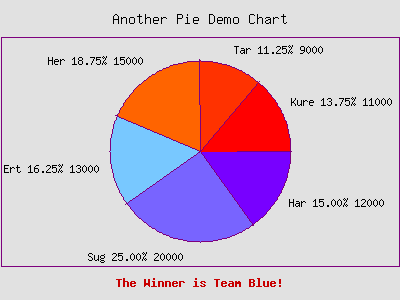
\includegraphics[scale = 0.6]{d_pie3.png}
	\end{center}
	\caption{Pie chart}
	\label{fig:pie}
\end{figure}
\begin{verbatim}
use Chart::Pie;

$g = Chart::Pie->new();

$g->add_dataset ('Har', 'Sug', 'Ert', 'Her', 'Tar', 'Kure');
$g->add_dataset (12000, 20000 , 13000, 15000, 9000, 11000  );

%opt = ( 'title' => 'Another Pie Demo Chart',
         'label_values' => 'both',
         'legend' => 'none',
         'text_space' => 10,
         'png_border' => 1,
         'graph_border' => 0,
         'colors' => { 'x_label' => 'red',
                       'misc' => 'plum',
                       'background' => 'grey',
                       'dataset0' => [120, 0, 255],
                       'dataset1' => [120, 100, 255],
                       'dataset2' => [120, 200, 255],
                       'dataset3' => [255, 100, 0],
                       'dataset4' => [255, 50, 0],
                       'dataset5' => [255, 0, 0],
                     },
         'x_label' => 'The Winner is Team Blue!',
        );

$g->set (%opt);

$g->png ("pie.png");
\end{verbatim}
\herv{Constructor:} An instance of a pie chart object can be created with the constructor new():\\
\fett{\$obj = Chart::Pie->new();}\\
\fett{\$obj = Chart::Pie->new(\kursiv{width}, \kursiv{height});}\\
\\
If \fett{new} has no arguments, the constructor returns an image with the size 300x400 pixels. If new has two arguments \kursiv{width} and \kursiv{height}, it returns an image with the desired size. \\ 
\\ 
\herv{Methods:}All universally valid methods, see page \pageref{methods}: Chart::Base. \\
\\
\herv{Attributes/Options:} All universally valid options, see page \pageref{options}. Also available, these special options:
\begin{description}
\item['label\_values'] Tells the pie chart what labels to draw beside the pie. Valid values are 'percent', 'value', 'both' and 'none'. Defaults to 'percent'.
\item['legend\_label\_values'] Tells the pie chart what labels to draw in the legend. Valid values are 'percent', 'value', 'both' and 'none'. Defaults to 'value'.
\end{description}